\section*{Time Series data \footnotesize\emph{Fabian Brix, Anton Ovchinnikov}}
The basis for the prediction part of this project are time series of price data. We acquired these for different stages of pricing in the supply chain and at different time granularities from different Indian government ministries. The data had to be downloaded and processed into usable formats from the websites of these ministries. The different sources consist of the Ministry of Agriculture and the Ministry of Trade and their various departments. In terms of different types of prices we differentiate between wholesale market prices and retail prices. We subsequently structure our documentation of data sources and the data processing according to these two types.

\subsection*{Wholesale prices}

\subsubsection*{Wholesale price index}
An index that measures and tracks the changes in price of goods in the stages before the retail level. Wholesale price indexes (WPIs) report monthly to show the average price changes of goods sold in bulk, and they are a group of the indicators that follow growth in the economy.\par
%(taken from investopedia.com)\\

\subsubsection*{Data sources}
We came across a \href{http://agmarknet.nic.in/}{website} maintained by the Indian Ministry of Agriculture that tracked \emph{daily} wholesale prices for units of 100 kilograms for a huge number of market places across the country. The data is recorded back to 2005 and is supplemented by stock arrival numbers.\par
Due to large amount of data available, as well as time and resources needed to pull it, we constrained ourselves to choosing several major products (Onion, Rice, Wheat, Apple, Banana, Coriander, Potato, Paddy(Dhan), Tomato), where a Python script was used to download all available data for the selected products directly from the website, using simple HTTP GET requests. Raw HTML data was then converted to CSV format with predefined structure and saved for later processing.

\subsection*{Retail prices}
\subsubsection*{Data sources}

\begin{itemize}

\item[1.] Daily retail prices

Daily retail prices were found at the \href{http://fcainfoweb.nic.in/}{website}, created by Department of Consumer Affairs of India. One can choose the type of report (price report, variation report, average/month end report) and the desired date, and then receive the requested data in HTML format. This website was used to query price reports from 2009 to 2014, for 59 cities and 22 products. Similar to the wholesale daily prices, raw HTML data was converted to CSV files in normalized format, which was intended to facilitate further processing.

\item[2.] Weekly retail prices

The \href{http://rpms.dacnet.nic.in/}{Retail Price Information System} of the Indian Ministry of Agriculture was queried to obtain weekly retail prices.\par
Unlike daily prices, the only available data format that was capable of being parsed, was Microsoft Excel .xls format. So all the required .xls files were downloaded using a Python script, and then 'xls2csv' was used to convert .xls documents to CSV data format. For some reason, the majority of product names were missing in the downloaded .xls files, so a basic heuristic, which involved the order of product names, was used to reconstruct the data.
The data obtained described information about prices for a large number of markets, around 60 products and hundreds of subproducts, dating back to 2005, but, unfortunately, the data was far from complete, especially for 2005-2007 time frame.

\end{itemize}

\subsection*{Price sequences \footnotesize\emph{Ching-Chia Wang}}
We used Pandas, a powerful and fast Python data analysis library, to load the csv files of datasets, to clean them up, and to organize them into usable formats. The prices of all products in these datasets are collected through a human reporting mechanism from local institutions to a central ministry. Due to the nature of this data collecting process, the qualities of these 3 datasets suffer from human neglects and mistakes. We thus need to conduct 2 phases of work prior to time series analysis and price prediction: data clean-up and dataset usability analysis.

\subsubsection*{Price Data Clean-up}
In data clean-up, we fixed several defects in the original datasets of the data sources. Each series originally has different portion of missing dates, and some have multiple data points of the same date with different values. The first stage of clean-up was to make each series align to a unique sequence of dates with constant date frequency by inserting NaNs to the missing and duplicated dates.

Next, we discovered that there are many outliers with extreme values in the series. For example, a price of 10 rupee today jumps to 100 tomorrow, and then goes back to 10 the day after. Such cases are more likely caused by human mistakes in reporting prices to the Indian ministries, so we used a heuristic to remove these suspicious spikes in the series. By taking the daily differences in percentage of a series, we were able to remove data points of the dates which perform more than 100\% price change in one time step (daily or weekly).

Finally, we patched the missing parts of the series with common methods such as linear or cubic spline interpolation.

\begin{figure}[!ht]
    \centering
        \begin{subfigure}[b]{.45\textwidth}
        \centering
        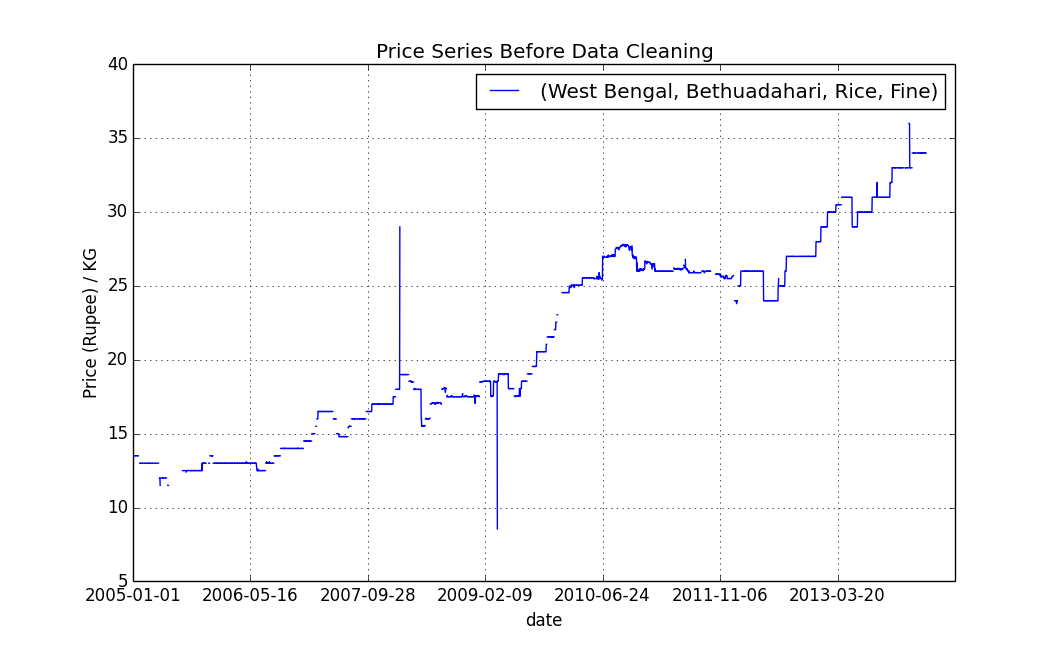
\includegraphics[width=\textwidth]{./img/before.png}
        \caption{Sample price series after date alignment during data cleaning}
        \label{subfig:sc1}
        \end{subfigure}
        \quad
        \begin{subfigure}[b]{.45\textwidth}
        \centering
        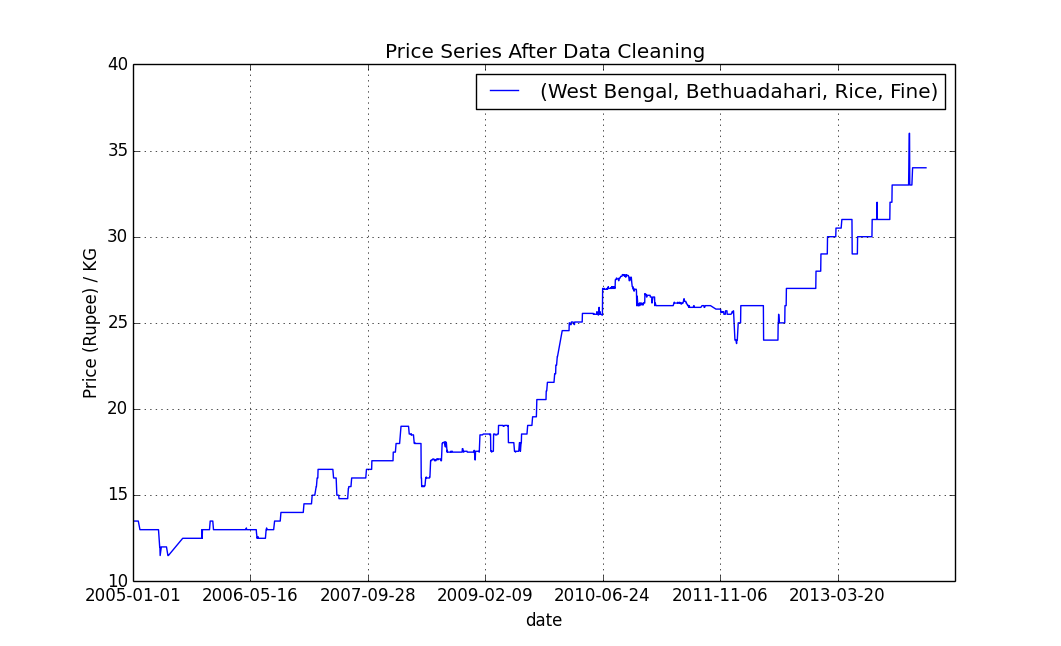
\includegraphics[width=\textwidth]{./img/after.png}
        \caption{Sample price series after spikes-removing and interpolation}
        \label{subfig:sc2}
        \end{subfigure}

    \caption{Example of time series cleaning process}
    \label{fig:series_cleaning}
\end{figure}

\subsubsection*{Price Dataset Usability Analysis}

The dataset usability analysis phase was intended to explore the data to find usable materials for analysis and prediction in later stages. We first filtered out all the series with less than 60\% of non-missing data, then computed some indicators of the data availability of each product in each region. Unfortunately, we have found out that all the datasets are far from satisfying.

The data availability in the daily wholesale dataset varies tremendously among different products and regions. Although there are about 15 regions, 7 candidate products, and more than 10 sub-categories for each product after filtering, most of the combinations of region, product, sub-category do not have enough available data for analysis and prediction. Fortunately, we did find out a few very good series which have more than 80\%~90\% of valid data and also perform the desired traits of high volatility and rising trend across time. These become good candidates for later analysis and prediction.

On the other hand, the daily retail dataset appears to have consistent data availability among products and regions, but in fact all products have only about 60\% of valid data in each region. Moreover, after examining each series via plots, we discovered that most of the daily retail series have weird behavior. For instance, the price of a series may have identical values for a long period and suddenly jump to another value, which makes the series look like levels of ladders. These series are not useful since such pattern is probably caused by dysfunctional price reporting process. Last, the weekly retail datatset has too many incorrect data points due to the heuristic of parsing excel files mentioned in the previous section. We thus concluded that the weekly retail dataset can be discarded with no loss.

Considering the limitations of the current price datasets, we have concluded the following potential usage of them: (1) Select a few representative series of each product with very good data quality. By using these individual series as a starting point of analysis and prediction, we can find out general characteristics and also the feasibility of predicting the prices of these highly volatile commodities. (2) Merge the series of the same product in each region to construct an extended dataset containing a uniform profile for each product in each region. In this way, we can gain a national overview of trends and price variations of different products.

\begin{figure}
    \centering
    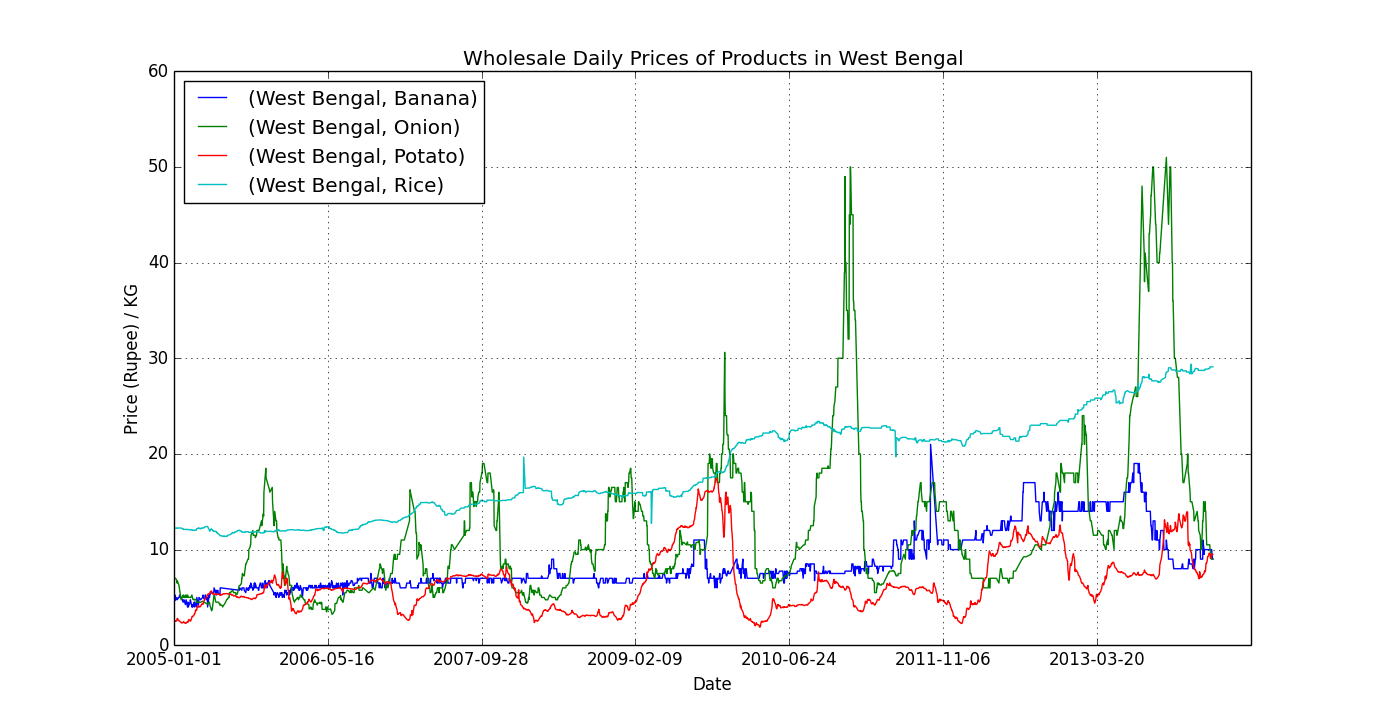
\includegraphics[width=.7\textwidth]{./img/merged_west_bengal_products.png}
    \caption{Merged series of foods in West Bengal from the wholesale daily dataset}
\end{figure}

\subsection*{Other sources \footnotesize\emph{Joseph Boyd}}
After some research we decided to include additional data that affects especially agricultural commodity prices such as the price of crude oil, climate data and the inflation in form of the Consumer Price Index (CPI). The monthly international price of crude oil was downloaded from a US government website. All other types of data were ``scraped'' from two online sources using HTML parsing library, `BeautifulSoup' for Python. The first of these sources was meteorological web site Tu Tiempo (http://www.tutiempo.net). Daily climate data (comprising temperature, humidity, perspiration etc.) for the last 16 years (1999-2014) was collected for over 100 locations in India. The script for this is get\_climate\_data.py. The second source was monthly inflation (CPI) data for India for the past 16 years from inflation.eu. The script for this purpose is get\_inflation\_data.py.
%exchange rate
%crude oil

\section*{Social Media data \footnotesize\emph{Joseph Boyd}}
For the other significant part of the project we decided to limit ourselves to a basic analysis of conversations on twitter. Originally we planned to also look into other platforms such as Facebook but quickly came to realize that the data publicly available through the API was of little use to us. Obtaining data from the twitter APIs turned out to be harder than expected and involved a number of heuristics. Twitter provides different APIs for different purposes. The two that are free are the Streaming API which allows real-time streaming of only 1\% of newly posted tweets. Since we wanted 'historical' tweets we had to find a workaround by using the REST API and getting tweets by user.\par
Twitter is a rich resource for studying cutting-edge trends on a global scale. Given a sufficiently large data collection effort, Twitter user discourse indicating changes in commodity prices may be obtained. This discourse supplies us with predictors The Humanitas project harvests huge amounts of user activity from this social media platform in order to capture the sparsely distributed activity pertaining to food prices. It is this aspect of the project which promotes it to the domain of `big data'.

\subsection*{Historical tweets}
\subsubsection*{Approach 1: Fetching "historical" tweets through Twitter API \footnotesize\emph{Joseph Boyd}}
Using the Twython package for python we are able to interface with the Twitter API. Our methodology (figure \ref{fig:methodology}) is to select the twitter accounts of a number of regional celebrities as starting points. These are likely to be `followed' by large numbers of local users. In a first phase (tweet\_collection.py.get\_followers()), from each of these sources we may extract a list of followers and filter by various characteristics. Once a substantial list has been constructed it must be merged (merge.py and remove\_intersection.py), we may proceed to download the tweet activity (up to the 3200 most recent tweets) of each of these users in a second phase (tweet\_collection.py.get\_tweets()).

Despite recent updates allowing developers greater access, Twitter still imposes troublesome constraints on the number of requests per unit time window (15 minutes) and, consequently, the data collection rate. It is therefore necessary to: 1) optimise the use of each request; and 2) parallelise the data collection effort.

As far as optimisation is concerned, the \textbf{GET statuses/user\_timeline} call may be called 300 times per 15 minute time window with up to 200 tweets returned per request. This sets a hard upper bound of 60000 tweets per time window. This is why the filtering stage of the first phase is so crucial. Using the \textbf{GET followers/list} call (30 calls/time window), we may discard in advance the majority of twitter users with low numbers of tweets (often zero), so as to avoid burning the limited user timeline requests on fruitless users, thus increasing the data collection rate. With this approach we may approach optimality and achieve 4-5 million tweets daily per process. However, it may be prudent to strike a balance between tweets per day and tweets per user. Therefore a nominal filter is currently set to 50 tweets minimum rather than 200. It is furthermore necessary to install dynamic time-tracking mechanisms within the source code so as to monitor the request rates and to impose a process `sleep' when required.

Parallelisation begins with obtaining N ($\approx 10$) sets of developer credentials from Twitter (https://dev.twitter.com/). These N credentials may then be used to launch N processes (get\_users.sh) collecting user data in parallel. Given the decision to divide the follower collection and tweet collection into separate phases (this may alternatively be done simultaneously), there is no need for distributed interaction between the processes to control overlap, as each process will simply take $1/N$ th of the follower list produced in phase 1 and process it accordingly. It should be relatively simple to initiate this parallel computation given the design of the scripts.

\begin{table}
\begin{center}
\begin{tabular}{ | c | c | c | c | c | }
\hline
Phase 1  \\ \hline
Users & Duration (s) & Sleep (s) & User Rate & Type \\ \hline
334 & 2795 & 2047 & - & Total \\ \hline
299 & 2700 & 2047 & 99.7 & Normalised (3 windows) \\ \hline
Phase 2 \\ \hline
Tweets (Users) & Duration (s) & Sleep (s) & Tweet Rate & Type \\ \hline
171990 (334) & 3108 & 922 & - & Total \\ \hline
150008 (309) & 2700 & 922 & 50002.7 &  Normalised (3 windows) \\ \hline
\end{tabular}
\end{center}
\caption{Trial run results}
\label{table:benchmark}
\end{table}

A benchmarking test (table \ref{table:benchmark}) was performed in order to support configuration choices for the parallelisation. The test involved collecting the tweets from all good users within the first 20000 followers of @KareenaOnline, the account of a local celebrity. The following observations can be made:

\begin{itemize}
\item only 1.5-2\% of users are considered "good" under the current choice of filters (location, min. 50 tweets etc.);
\item Despite different levels of sleeping, phase 2 reads from users at roughly the same rate that phase 1 collects them (approximately 100 per time window in both cases);
\item Phase 2 produces around 50000 tweets per time window.
\end{itemize}

It is important to note however, that the rate of "good" users increases varies depending on the notoriety of the source account outside of India. To ensure good coverage for user collection, a wide variety of source users was chosen including rival politicians, musicians, sportspersons, film stars, journalists and entrepreneurs.

Tweet collection for Humanitas occurred in two main waves. In the first wave 180 000 users identifiers were collected. This amounted to 110 million tweets, collected over about three days, totalling 288GB of information (note a tweet response comprises the textual content as well as a substantial amount of meta data). In second wave of collection we encountered the effect of diminishing returns as many of the newly harvested users had already featured in the first wave. Despite a lengthier collection effort, only 110 000 new users were collected, leading to 70 million additional tweets and a grand total for the two waves of about 500GB of data. Future collection work for Humanitas would benefit from a more sophisticated approach to collecting users (phase 1), for example, by constructing a Twitter user graph.

\begin{figure}
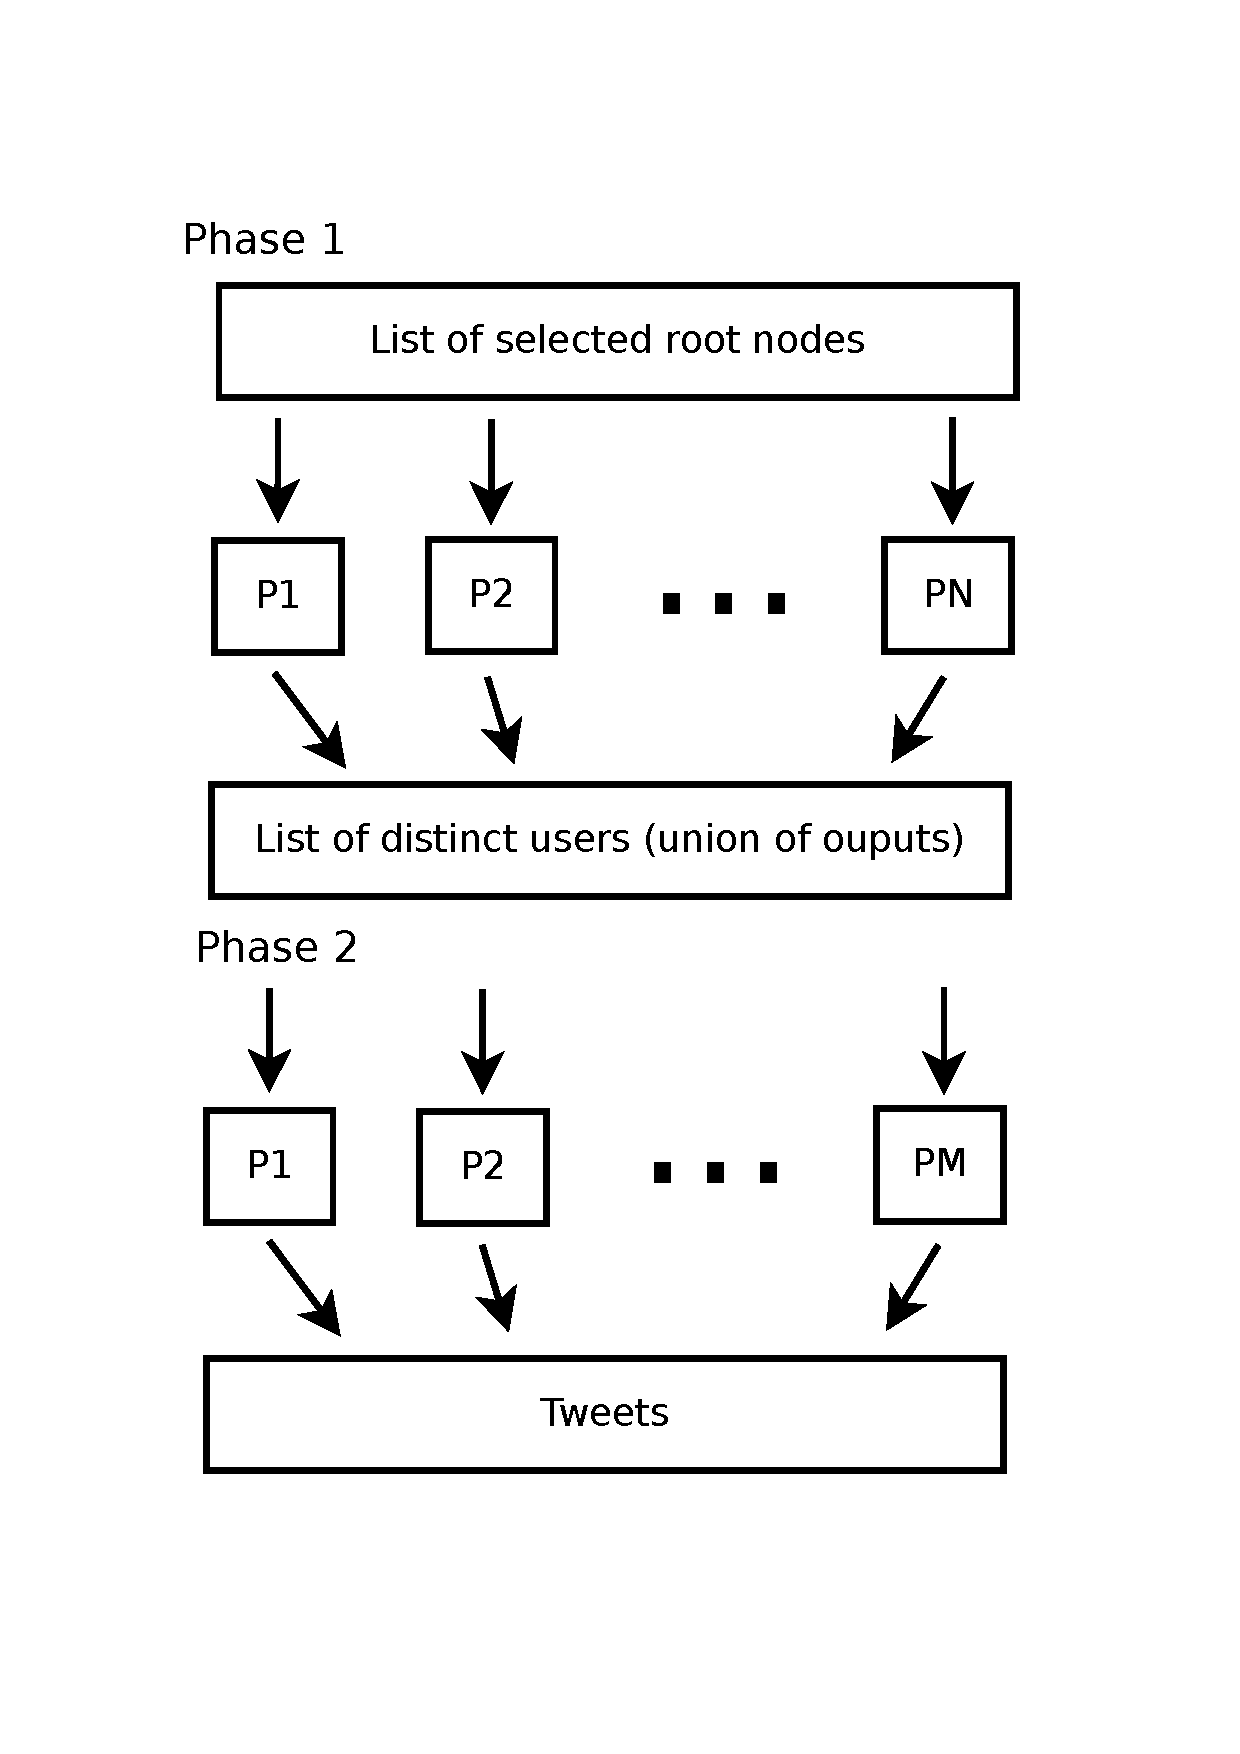
\includegraphics[width=.7\textwidth]{./img/CollectionProcess.pdf}
\caption{Tweet collection methodology.}
\label{fig:methodology}
\end{figure}

\subsubsection*{Approach 2: Filtering tweets provided by webarchive.org}
\emph{Gabriel Grill} \\
Before we were sure to get tweets from the twitter APIs we explored a set of archive files made available on \href{https://archive.org/details/twitterstream}{archive.org}. These archives were recorded via the twitter Streaming API and aggregated by month.
They contain contain 1\% of all tweets from 2011 to 2013 (not only India!). The collection of tweets was done via a python script which was executed on all 8 Azure nodes in parallel. Beforehand the respective archives were downloaded to the nodes with a download speed of approx. 20 MB/s. The storage was to our surprise no problem, because every Azure node gets 133 GB of temporal storage for disposal. About 550 GB of compressed tweets were processed and filtered in about 36 hours per node.
\newline
The applied filter got rid of tweets not containing at least one food commodity specific word (e.g. rice, curry, food, ...) and one predictive word (e.g. increase, decrease, price, ...). Also Retweets were filtered out, because sophisticated duplicate detection across 8 nodes can be costly and some exploration of the data showed that almost all duplicates were filtered out with this simple check. Since we want to predict food prices for certain regions, the location of the tweets is very important. We came up with a simple scheme to detect locations:
\begin{itemize}
\item \textbf{Geo-location:} Some tweet objects contain a field 'coords' which states the exact location coordinates the tweet was sent from.
\item \textbf{Mentioned regions:} In the associated tweet text regions can be mentioned, which can also give clues on the regions affected.
\item \textbf{Places:} When submitting a tweet an user can also specify a place associated with the tweet. This information can be extracted from the tweet objects.
\item \textbf{User location:} Most tweets objects also have an associated user object, which contains a user location sometimes. The textual information of this field is tokenized and compared with a list of known regions.
\end{itemize}
According to the categories mentioned above, the tweets were split up in several files. Since the \emph{Approach 1.} conveyed much more tweets, the archive sample was only used for data exploration and testing of the more refined tweet processing.

\subsubsection*{Daily tweet aggregator}
\emph{Gabriel Grill} \\
Our first idea was to build a continuously running process, which fetches the newest data from the twitter stream from India. But after applying a simple filter, we came to the conclusion that the data is to sparse for this approach, since the 'Twitter Streaming API' supplies only 1\% of all available tweets. Since the amount of twitter users in India is rapidly growing, this could be a promising approach for the future.

\subsubsection*{Clustering according to keywords}
\emph{Gabriel Grill} \\
Since relevant data was really sparse, we didn't expect much gain from any unsupervised learning techniques and decided to omit clustering. Instead we decided to manually explore a sample of the tweet data and create a list of indicator words used for detecting e.g. poverty, price in/decrease, sentiment and so on. Doing occurrence checks for all crafted words and storing the result, yields feature vectors for every tweet usable for prediction.

\subsubsection*{Issue of storage}
\emph{Gabriel Grill} \\
At first we believed that there wouldn't be enough space to store all tweets, but after setting up an azure node, we found that there is about 133 GB of temporal storage associated with it. We used this space to store the huge amount of tweets, but since the storage is temporal we lost tweets several times. This was due to configuration mistakes by us and Azure's 'healing'. When Azure detects anomalies, internal errors or just that it has to move images around, affected nodes are restarted, which results in a loss of tweets for us. Because of that, all filtered tweets were later stored on the main disk to avoid future losses.

\subsection*{Issue of localization}
\emph{Gabriel Grill} \\
It's was very important for us to detect the location of tweets, because we wanted to predict volatile food prices at regional granularity. Since Twitter is not widespread in India and localized tweets are rare, we had to come up with heuristics to deal with that.

\subsubsection*{Geolocalized tweets}
Filtering the available archives of tweets taken from the API yielded near to no geolocalized tweets from India matching our set of keywords. The reason is evident, because the twitter API only allows extraction of 1\% of tweets and only 2\% of tweets are actually geolocalized. In effect, getting tweets that match our keywords specific to food commodities is very unlikely. We had more luck with tweets from Indonesia, however as already explained we were unable to attain enough price sequences from Indonesia to actually train a model. Furthermore, the time constraints didn't allow us to get tweets from India and Indonesia in parallel in order to do some "stand-alone" clustering analysis.

\subsubsection*{Approximation: Mapping tweets to user location}
\emph{Gabriel Grill} \\
To get as many tweets as possible associated with a location we decided to use the locations of user accounts as a simple heuristic. We created a mapping between city and region names and used to to identify valid locations, which were then used during later processing.

\section*{Processing}
After all tweets were collected, we had to process and reformat their content for the neural networks (prediction) and the web visualisation.

\subsection*{Crafting indicators from tweets}
\emph{Gabriel Grill} \\
To use the collected tweets for prediction in the neural network, aggregated indicators had to be extracted from the collection. The final result of this processing was then stored in \emph{csv} files.
\\ \\
Every word occurrence check (either for filtering or feature extraction) in tweet texts was done by iterating over the list of tokens generated from the text. Several NLP techniques were used to improve the word comparison. For every tweet a category/indicator counter was kept to keep track of the number of occurrence of certain predictive words. The processed tweets and their extracted features (indicator counts) were stored in a Cassandra cluster and later queried with Shark. The result of the shark queries was then converted to \emph{csv} files.

\subsubsection*{Sentiment analysis}
\emph{Anton Ovchinnikov} \\
Sentiment analysis, or opinion mining, is the concept of using different computer science techniques (mainly machine learning and natural language processing) in order to extract sentiment information and subjective opinions from the data. In our context this may help us to find out how circumstances in relation to commodity prices affect the overall mood in the population.

From the start we decided that we did not want to build our own sentiment analysis system since the proper implementation, testing and evaluation would require a considerable effort compared with the total project workload. Instead, we are planning to use some of already developed solutions and tune them to our needs.
\newline \newline
Several sentiment analysis frameworks were tested, including:

\begin{itemize}
\item SentiStrength \par (http://sentistrength.wlv.ac.uk/)

\item Stanford CoreNLP \par (http://nlp.stanford.edu/sentiment/code.html)

\item 'Pattern' library from the University of Antwerp \par (http://www.clips.ua.ac.be/pages/pattern-en)
\end{itemize}
All of these software packages produced reasonable results on some short and simple sentences, but sentiment grades looked almost random on a set of real collected tweets. Most likely, factors such as misspelled words, acronyms, usage of slang and irony contributed to the overall ambiguity of sentiment grades assignment.
\newline \newline
Therefore, we decided to build and use our own simple system, which incorporated basic natural language processing and opinion mining techniques, but was mainly focused on extracting relevant keywords, which could help to estimate tweets from the specific point of view. This approach, which also takes into account issues originating from word misspelling, is described in next two paragraphs.

\subsubsection*{Extracting predictor categories}
\emph{Anton Ovchinnikov} \\
First, several "predictor categories" were selected. These categories represent different aspects of price variation, and each category includes several sets of words of different polarities. For example, the category \emph{"price"} has two polarities: \emph{"high"} and \emph{"low"}.
\\
The following word list belongs to \emph{"high"} polarity:

\emph{'high', 'expensive', 'costly', 'pricey', 'overpriced'},
\\
and these are words from \emph{"low"} list:

\emph{'low', 'low-cost', 'cheap', 'low-budget', 'dirt-cheap', 'bargain'}.
\\ \\
Likewise, a category "supply" has "high" polarity:

\emph{'available', 'full', 'enough', 'sustain', 'access', 'convenient'},
\\
and "low":

\emph{'run-out', 'empty', 'depleted', 'rotting'}.
\\ \\ \\
The dictionary with a total of 6 categories (each having at least two polarity word lists) was built (\emph{"predict", "price", "sentiment", "poverty", "needs", "supply"}), let's call it $D$.
\\ \\
Then, for each tweet a feature vector is built, representing the amount of words from each category and polarity. Several cases have to be taken into account. First of all, a word may be not in its base form ("price" -> "prices", "increase" -> "increasing"), which will prevent an incoming word from matching one from $D$. Therefore, we use stemming technique to reduce each word to its stem (or root) form. Another problem is misspelled words ("increase" -> "incrase", "incraese"), and for tweets it happens more than usual due to widespread use of mobile devices with tiny keyboards. Our solution to this problem is covered in the next section.

Here is the overview of predictor category extraction algorithms we implemented:\\ \\
\textbf{Preprocessing}: For each relevant word in $D$ a stem is computed using the Lancaster stemming method, and the stem is added to reverse index $RI$, which maps a stem to a tuple: (category, polarity). \\

\textbf{function get\_category(w):}

\indent
\begin{algorithm}[H]
Compute a stem $s$ from $w$ \par
Check if $s$ is present in $RI$.

  \eIf{yes}{
	\textbf{return} the corresponding tuple.
   }{
		ask spell checker for a suggestion \par
		is suggestion stem returned? \par
		\eIf{yes}{
			\textbf{return} the corresponding tuple from $RI$
		}{
			\textbf{return} None;
		}
  	}
% \caption{Algo}
\end{algorithm}
\noindent \\

On a high level, every tweet is split into words, and then each word (token) is passed through 'get\_category' function. But here's another problem we face using this approach: each relevant word we encounter may have a negation word (particle) before it, which subverts the meaning: "increases" -> "doesn't increase", "have food" -> "have no food", etc. To deal with this problem, we employed the following method: we added a special 'negation' category with a list of negation words ("not", "haven't", "won't", etc.), and if there is a word with "negative" category before some relative word (to be more precise, within some constant distance from it, say 2), then we change the polarity of relative word's category. For example, if a word is from category "poverty" and has "high" polarity (like "starving"), then negative category word right before it (such as "aren't") will turn the polarity to "low".


\subsubsection*{Tweets spell checking}
\emph{Anton Ovchinnikov} \\
People often do not pay much attention about the proper word spelling while communicating over the Internet and using social networks, but misspelled words may introduce mistakes in processing pipeline and significantly reduce the amount of filtered tweets, since the relevant, but incorrectly written word might not be recognized by the algorithm.

Several spell checking libraries were checked (Aspell and Enchant to name a few), but their 'suggest' method lacked both performance (several seconds to generate a suggestion for thousands words, which is very slow) and flexibility (it's not possible to specify the number of generated suggestions, as well as a threshold, such as maximal edit distance between words). Therefore, we decided to use a simple approach which involved computing edit distances between a given word and words from predictor categories dictionary ($D$).
\\
For each given word $w$ we compute its stem $s$ and then edit distance (also known as Levenshtein distance) to each word (stem) from $D$. It can be done really fast thanks to C extensions of \textit{python-levenshtein} module.
\\
After that, we choose the stem with minimal edit distance (using heap to store the correspondence between distances and words and to speed up selection of the minimal one), and check if the resulting number of "errors" (which is equal to distance) is excusable for the length of word $w$. For example, we don't allow errors for words of length 5 or less, only one error is allowed for lengths from 6 to 8, etc. If everything is alright, then the suggestion is returned, otherwise the word is discarded.

The approach proved to be fast and tweakable, and was successfully used for tweets processing.

\subsection*{Generation of time series}
\emph{Gabriel Grill} \\
All these indicators are crafted into a single time series of the form \emph{'Product', 'date', 'region', 'indicator1', ... , 'indicatorN'} via Shark queries. These indicators represent the amount of tweets matching a certain predictive category (as mentioned previously) normalized by the total amount of tweets mentioning the product that day. If a tweet is part of multiple categories, it's not clear what the intention behind the tweet was. That's why, as heuristic, we divide the sum of mentions of each predictive category by the total amount of identified mentioned categories for that tweet. We have a script to generate queries for all products and a script to parse the output into \emph{csv} format. The figure \ref{fig:architecture} illustrates the whole processing pipeline and gives a good overview of the architecture at the same time as well.

\begin{figure}
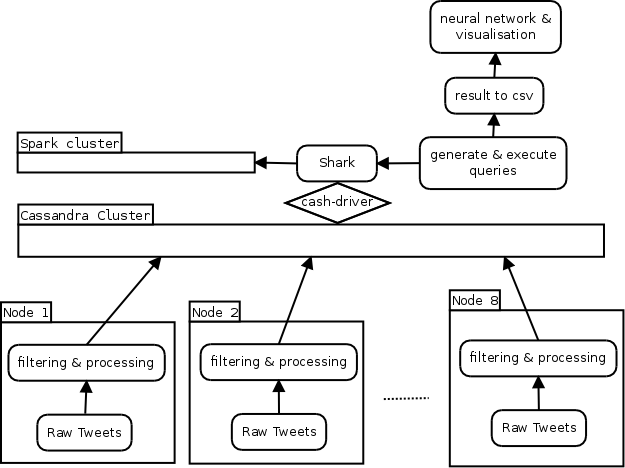
\includegraphics[width=.7\textwidth]{./img/architecture.png}
\caption{Tweet processing pipeline.}
\label{fig:architecture}
\end{figure}

\subsection*{Infrastructure \& Architecture}
\emph{Gabriel Grill} \\
Almost all downloading and processing of tweets was done in parallel on 8 Azure nodes. A script was written to upload public keys to the nodes for seamless access. The same script was used to execute various task on all or specific nodes. To handle the huge amounts of data and do efficient OLAP, we decided to use spark/shark. The data was first stored on each node separately on disk, then processed and afterwards inserted into a Cassandra DB cluster running on the nodes. The Apache Cassandra project is open source implementation of a NoSQL, column-oriented data base. It's known for being fault tolerant, which was very useful during various restarts, and processing many inserts fast. Since we had very limited memory on the non-temporal disk, we experienced 'Out of memory' errors, but because all data has been uploaded to the whole cluster, the scripts could continue running smoothly although some nodes were down. We also experienced node faults whenever the Azure node management 'healed' nodes.

Setting up the Cassandra cluster across multiple Azure subscriptions was tiring, since all used ports had to be opened on all machines manually via the Azure management web interface. Opening ports was regretfully not enough to get a fully functioning Spark cluster running, because Spark uses random ports for communication between running jobs. We tried setting up a VPN, but decided to quit after several hours due to time constraints and because it was not essential for the result that the Spark cluster had to be made up of all nodes. Luckily Shark on top of Spark with only one node was still fully functional and executed queries at reasonable speed. To connect Shark with Cassandra we used the 'Hive support for Cassandra' driver \emph{cash} by tuplejump. We experienced several problems (some undocumented) while installing (e.g. libraries missing, wrong paths, ...), but still managed to get it running. To improve speed between the nodes all VMs were created in the same region.
